%%%%%%%%%%%%%%%%%%%%%%%%%%%%%%%%%%%%%%%%%
% Beamer Presentation
% LaTeX Template
% Version 1.0 (10/11/12)
%
% This template has been downloaded from:
% http://www.LaTeXTemplates.com
%
% License:
% CC BY-NC-SA 3.0 (http://creativecommons.org/licenses/by-nc-sa/3.0/)
%
%%%%%%%%%%%%%%%%%%%%%%%%%%%%%%%%%%%%%%%%%

%----------------------------------------------------------------------------------------
%	PACKAGES AND THEMES
%----------------------------------------------------------------------------------------

\documentclass{beamer}

\mode<presentation> {

% The Beamer class comes with a number of default slide themes
% which change the colors and layouts of slides. Below this is a list
% of all the themes, uncomment each in turn to see what they look like.

%\usetheme{default}
%\usetheme{AnnArbor}
%\usetheme{Antibes}
%\usetheme{Bergen}
%\usetheme{Berkeley}
%\usetheme{Berlin}
%\usetheme{Boadilla}
%\usetheme{CambridgeUS}
%\usetheme{Copenhagen}
%\usetheme{Darmstadt}
%\usetheme{Dresden}
%\usetheme{Frankfurt}
%\usetheme{Goettingen}
%\usetheme{Hannover}
%\usetheme{Ilmenau}
%\usetheme{JuanLesPins}
%\usetheme{Luebeck}
\usetheme{Madrid}
%\usetheme{Malmoe}
%\usetheme{Marburg}
%\usetheme{Montpellier}
%\usetheme{PaloAlto}
%\usetheme{Pittsburgh}
%\usetheme{Rochester}
%\usetheme{Singapore}
%\usetheme{Szeged}
%\usetheme{Warsaw}

% As well as themes, the Beamer class has a number of color themes
% for any slide theme. Uncomment each of these in turn to see how it
% changes the colors of your current slide theme.

%\usecolortheme{albatross}
%\usecolortheme{beaver}
%\usecolortheme{beetle}
%\usecolortheme{crane}
%\usecolortheme{dolphin}
%\usecolortheme{dove}
%\usecolortheme{fly}
%\usecolortheme{lily}
%\usecolortheme{orchid}
%\usecolortheme{rose}
%\usecolortheme{seagull}
%\usecolortheme{seahorse}
%\usecolortheme{whale}
%\usecolortheme{wolverine}

%\setbeamertemplate{footline} % To remove the footer line in all slides uncomment this line
%\setbeamertemplate{footline}[page number] % To replace the footer line in all slides with a simple slide count uncomment this line

%\setbeamertemplate{navigation symbols}{} % To remove the navigation symbols from the bottom of all slides uncomment this line
}

\usepackage{graphicx} % Allows including images
\usepackage{booktabs} % Allows the use of \toprule, \midrule and \bottomrule in tables
\bibliographystyle{IEEEtran}

%----------------------------------------------------------------------------------------
%	TITLE PAGE
%----------------------------------------------------------------------------------------

\title[SLAM Baseline]{Simultaneous Localization and Mapping (SLAM) Baseline} % The short title appears at the bottom of every slide, the full title is only on the title page

\author{Assylbek Dakibay} % Your name
\institute[University of Waterloo] % Your institution as it will appear on the bottom of every slide, may be shorthand to save space
{
University of Waterloo \\ % Your institution for the title page
\medskip
\textit{dakibay@gmail.com} % Your email address
}
\date{\today} % Date, can be changed to a custom date

\begin{document}

\begin{frame}
\titlepage % Print the title page as the first slide
\end{frame}

\begin{frame}
\frametitle{Overview} % Table of contents slide, comment this block out to remove it
\tableofcontents % Throughout your presentation, if you choose to use \section{} and \subsection{} commands, these will automatically be printed on this slide as an overview of your presentation
\end{frame}

%----------------------------------------------------------------------------------------
%	PRESENTATION SLIDES
%----------------------------------------------------------------------------------------
\section{LSD SLAM}
\begin{frame}
\frametitle{Large Scale Direct SLAM}
\begin{tabular}{cl}  
         \begin{tabular}{c}
           \includegraphics[height=4cm, width=7cm]{figs/LSD_SLAM.png}
           \end{tabular}
           & \begin{tabular}{l}
             \parbox{0.3\linewidth}{%  change the parbox width as appropiate
             \tiny{\textbf{Large Scale Direct (LSD) Monocular SLAM Process} Featureless SLAM algorithm that can be run in real time on a CPU \cite{engel2014lsd}.}
    }
         \end{tabular}  \\
         \end{tabular}
\end{frame}
%
%%------------------------------------------------
%
\begin{frame}

\frametitle{SVO}
\begin{columns}[c] % The "c" option specifies centered vertical alignment while the "t" option is used for top vertical alignment

\column{.45\textwidth} % Left column and width
\tiny{\textbf{Loop Closure} Generated maps for outdoors environment before and after loop closure \cite{engel2014lsd}. }  
\column{.5\textwidth} % Right column and width
\begin{figure}
\includegraphics[height=7cm, width=6cm]{figs/Loop_closure.png}	
\end{figure}
\end{columns}




\end{frame}


\begin{frame}
\frametitle{LSD SLAM On MAV}
\begin{columns}[c] % The "c" option specifies centered vertical alignment while the "t" option is used for top vertical alignment

\column{.25\textwidth} % Left column and width
\tiny{\textbf{LSD SLAM using MAV } Micro Aerial Vehicle (Parrot Bebop).  Ultrasonic and air pressure sensors are used for improving scale measurements  \cite{von2016autonomous}.}
\column{.5\textwidth} % Right column and width
\begin{figure}
\includegraphics[height=7cm, width=7cm]{figs/LSD_bebop.png}	
\end{figure}
\end{columns}
\end{frame}
%
%%------------------------------------------------
%
\section{Semi-Direct Visual Odometry}
\begin{frame}
\frametitle{SVO}
\begin{columns}[c] % The "c" option specifies centered vertical alignment while the "t" option is used for top vertical alignment

\column{.45\textwidth} % Left column and width
\tiny{\textbf{Fast Semi-Direct Visual Odometry (SVO)} The SVO process \cite{forster2014svo}.}
\column{.5\textwidth} % Right column and width
\begin{figure}
\includegraphics[height=7cm, width=6cm]{figs/SVO_pipeline.png}	
\end{figure}
\end{columns}
\end{frame}

\begin{frame}
\frametitle{Multiple Columns}
\begin{columns}[c] % The "c" option specifies centered vertical alignment while the "t" option is used for top vertical alignment

\column{.25\textwidth} % Left column and width
\tiny{\textbf{Fast Semi-Direct Visual Odometry (SVO) Results} The SVO Mapping results for outdoors environment using a Micro Aerial Vehicle \cite{forster2014svo}.}
\column{.5\textwidth} % Right column and width
\begin{figure}
\includegraphics[height=7cm, width=7cm]{figs/SVO_results.png}	
\end{figure}
\end{columns}
\end{frame}



%
%%------------------------------------------------
%\section{Second Section}
%%------------------------------------------------
%
%\begin{frame}
%\frametitle{Table}
%\begin{figure}
%	\vspace{1pt}
%
%	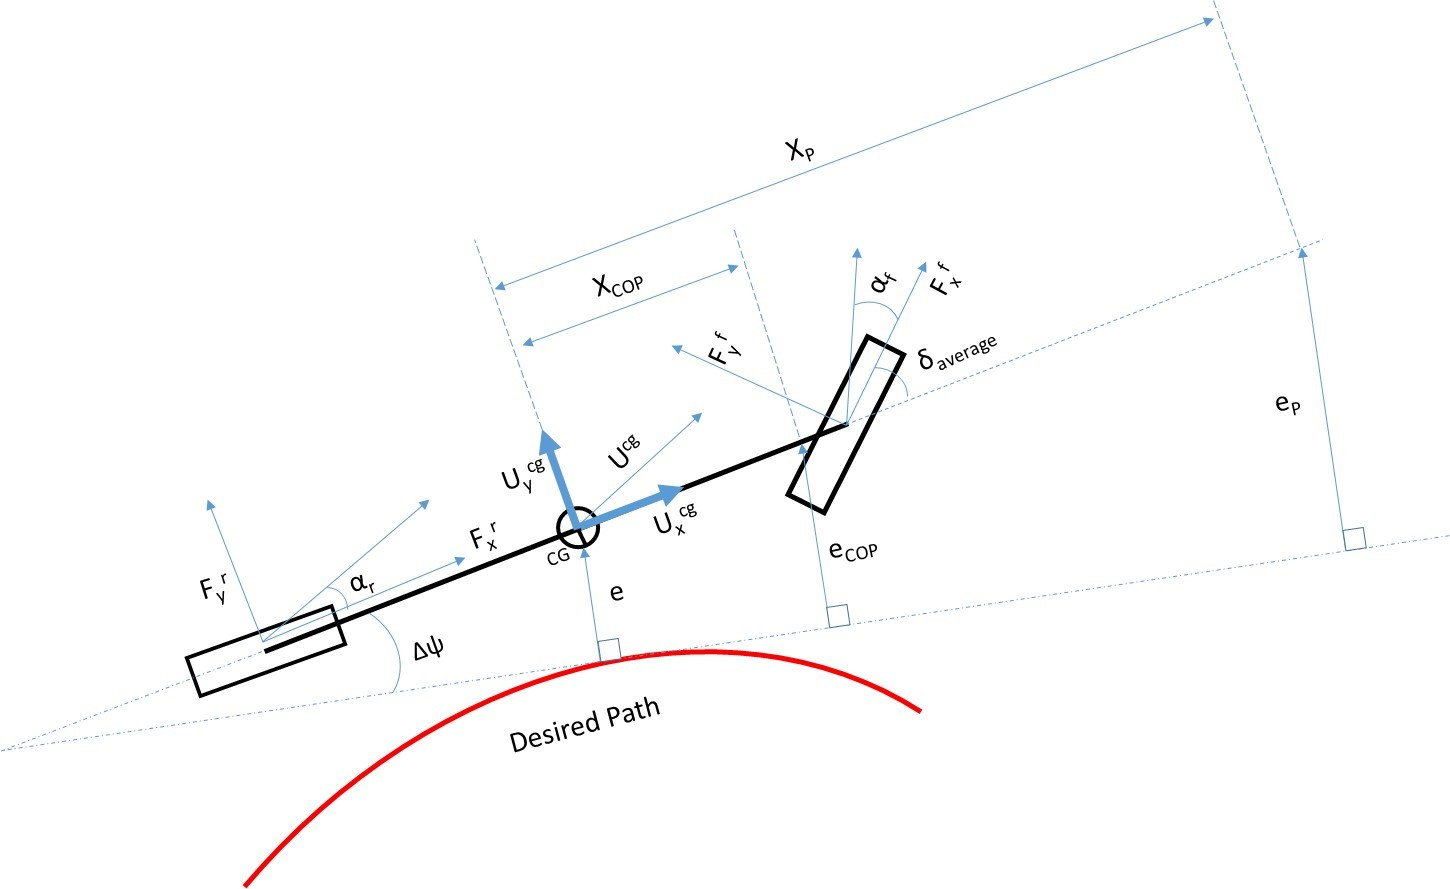
\includegraphics[width = .5 \linewidth]{figures/controller_diagram.jpg}
%
%	\caption{potential field controller diagram model}
%  	\label{fig:controller_diagram}
%\end{figure}
%\end{frame}
%
%%------------------------------------------------
%
%\begin{frame}
%\frametitle{Theorem}
%\begin{theorem}[Mass--energy equivalence]
%$E = mc^2$
%\end{theorem}
%\end{frame}
%
%%------------------------------------------------
%
%\begin{frame}[fragile] % Need to use the fragile option when verbatim is used in the slide
%\frametitle{Verbatim}
%\begin{example}[Theorem Slide Code]
%\begin{verbatim}
%\begin{frame}
%\frametitle{Theorem}
%\begin{theorem}[Mass--energy equivalence]
%$E = mc^2$
%\end{theorem}
%\end{frame}\end{verbatim}
%\end{example}
%\end{frame}
%
%%------------------------------------------------
%
%\begin{frame}
%\frametitle{Figure}
%Uncomment the code on this slide to include your own image from the same directory as the template .TeX file.
%%\begin{figure}
%%\includegraphics[width=0.8\linewidth]{test}
%%\end{figure}
%\end{frame}
%
%%------------------------------------------------
%
%\begin{frame}[fragile] % Need to use the fragile option when verbatim is used in the slide
%\frametitle{Citation}
%An example of the \verb|\cite| command to cite within the presentation:\\~
%
%This statement requires citation \cite{p1}.
%\end{frame}
%
%%------------------------------------------------
%
%\begin{frame}
%\frametitle{References}
%\footnotesize{
%\begin{thebibliography}{99} % Beamer does not support BibTeX so references must be inserted manually as below
%\bibitem[Smith, 2012]{p1} John Smith (2012)
%\newblock Title of the publication
%\newblock \emph{Journal Name} 12(3), 45 -- 678.
%\end{thebibliography}
%}
%\end{frame}
%
%%------------------------------------------------

\begin{frame}

\bibliography{presentation_slam}
\end{frame}

%----------------------------------------------------------------------------------------

\end{document} 